\chapter{Resultater}
Denne sektion har til formål at præsentere opgavens resultater. For at evaluere metoderne, er en måling for metodernes repeterbarhed opstillet, der udtrykker forholdet imellem korrekte korrespondancer og middelværdien af det samlede antal interessepunkter fundet i begge billeder \cite{eval}:
\begin{equation}
r_{I_1,I_2)}=\dfrac{C(I_1,I_2)}{\text{mean}(n_1,n_2)}
\end{equation}
hvor $C(I_1,I_2)$ angiver antallet af korrekte korrespondancer imellem to billeder og $n_1=\bold{|A|}$ og $n_2=\bold{|A'|}$.
%$\text{mean}(\bold{|P_1|},\bold{|P_2|)}$ angiver middelværdien af det samlede antal af fundne interessepunkter i det to billeder
%<beskriv hvordan punkter fjernes>
Moravec og Harris er blevet modificeret, for at få dem til at passe med SIFT. I begge tilfælde foldes billederne med en Gausskerne, og nedskaleres efter $\sigma$, som illustreret figur <???>, hvorefter detektionsmetoderne anvendes. 
\\
\\
I nedenstående tabeller angiver Filename $x$ filnavnene på de billeder der er fundet korrespondancer mellem. $|A|$ og $|A'|$ er defineret som i afsnit 3.5. $Match(A, A')$ er antallet af fundne korresponderende punkter, givet matching algoritmen fra afsnit 5.5. Givet det store antal matchende punkter, er det her antaget, at alle punkter fundet ved $Match$ algoritmen er sande positiver <korrekte korrespondancer> - mere om dette er omtalt i diskussionen af resultaterne. De 15 bedste matches, er også vedlagt som billede, for hver metode <de kan findes i fuld størrelse i..>
\\
\\
De resultater der her er fremlagt og senere diskuteres, er fra en enkelt skala, fra en enkelt oktav. SIFT og SURF søger oprindeligt efter blobs i flere skalrum - disse udregninger indgår ikke i resultat sektionen. Denne beslutning er taget på baggrunden af rationalet, at markbilleder taget af en drone fra en bestemt kendt højde, skaber blobs af en bestemt størrelse. Det er derfor ikke nødvendigt at kigge efter blobs på andre skaler, end den, der empirisk har vist sig at give de bedste resultater  ved en forudgående undersøgelse.
\section{Moravec}
\section{Harris}


\begin{figure}[H]
    \centering
    \begin{center}    
    \begin{tabular}{ | l | l | l | l | l | l | l |}
    \hline
    Filename 1 & Filename 1 & |$\bold{A}$| & |$\bold{A'}$| & $mean(A,A')$ & $Match(\bold{A}, \bold{A}')$ & $Rm$ \\ \hline
IMG\_9370.jpg &	IMG\_9371.jpg &	4327 &	2616 &	3471.5 &	563 &	0.1621\\ \hline
IMG\_9371.jpg &	IMG\_9372.jpg &	2616 &	1842 &	2229.0 &	389 &	0.1745\\ \hline
IMG\_9372.jpg &	IMG\_9373.jpg &	1842 &	4376 &	3109.0 &	182 &	0.0585\\ \hline
IMG\_9373.jpg &	IMG\_9374.jpg &	4376 &	1873 &	3124.5 &	233 &	0.0745\\ \hline
IMG\_9374.jpg &	IMG\_9375.jpg &	1873 &	972 &	1422.5 &	172 &	0.1209\\ \hline
IMG\_9375.jpg &	IMG\_9376.jpg &	972 &	1429 &	1200.5 &	238 &	0.1982\\ \hline
IMG\_9376.jpg &	IMG\_9377.jpg &	1429 &	4036 &	2732.5 &	367 &	0.1343\\ \hline
IMG\_9377.jpg &	IMG\_9378.jpg &	4036 &	2760 &	3398.0 &	455 &	0.1339\\ \hline
IMG\_9378.jpg &	IMG\_9379.jpg &	2760 &	688 &	1724.0 &	376 &	0.2180\\ \hline
IMG\_9379.jpg &	IMG\_9380.jpg &	688 &	1154 &	921.0  &	212 &	0.2301\\ \hline
    \end{tabular}       
    \caption{\textcolor{gray}{\footnotesize \textit{Fire forskellige oktaver, og filterstørrelse, for et andenafledt filter}}}
    \label{tab:HARRISOCTAVE2}
     \end{center}
     \vspace{-2.5em}
\end{figure} \noindent
Middelværdi af repeatability mesaure  = 0.1505


\begin{figure}[H]
    \centering
    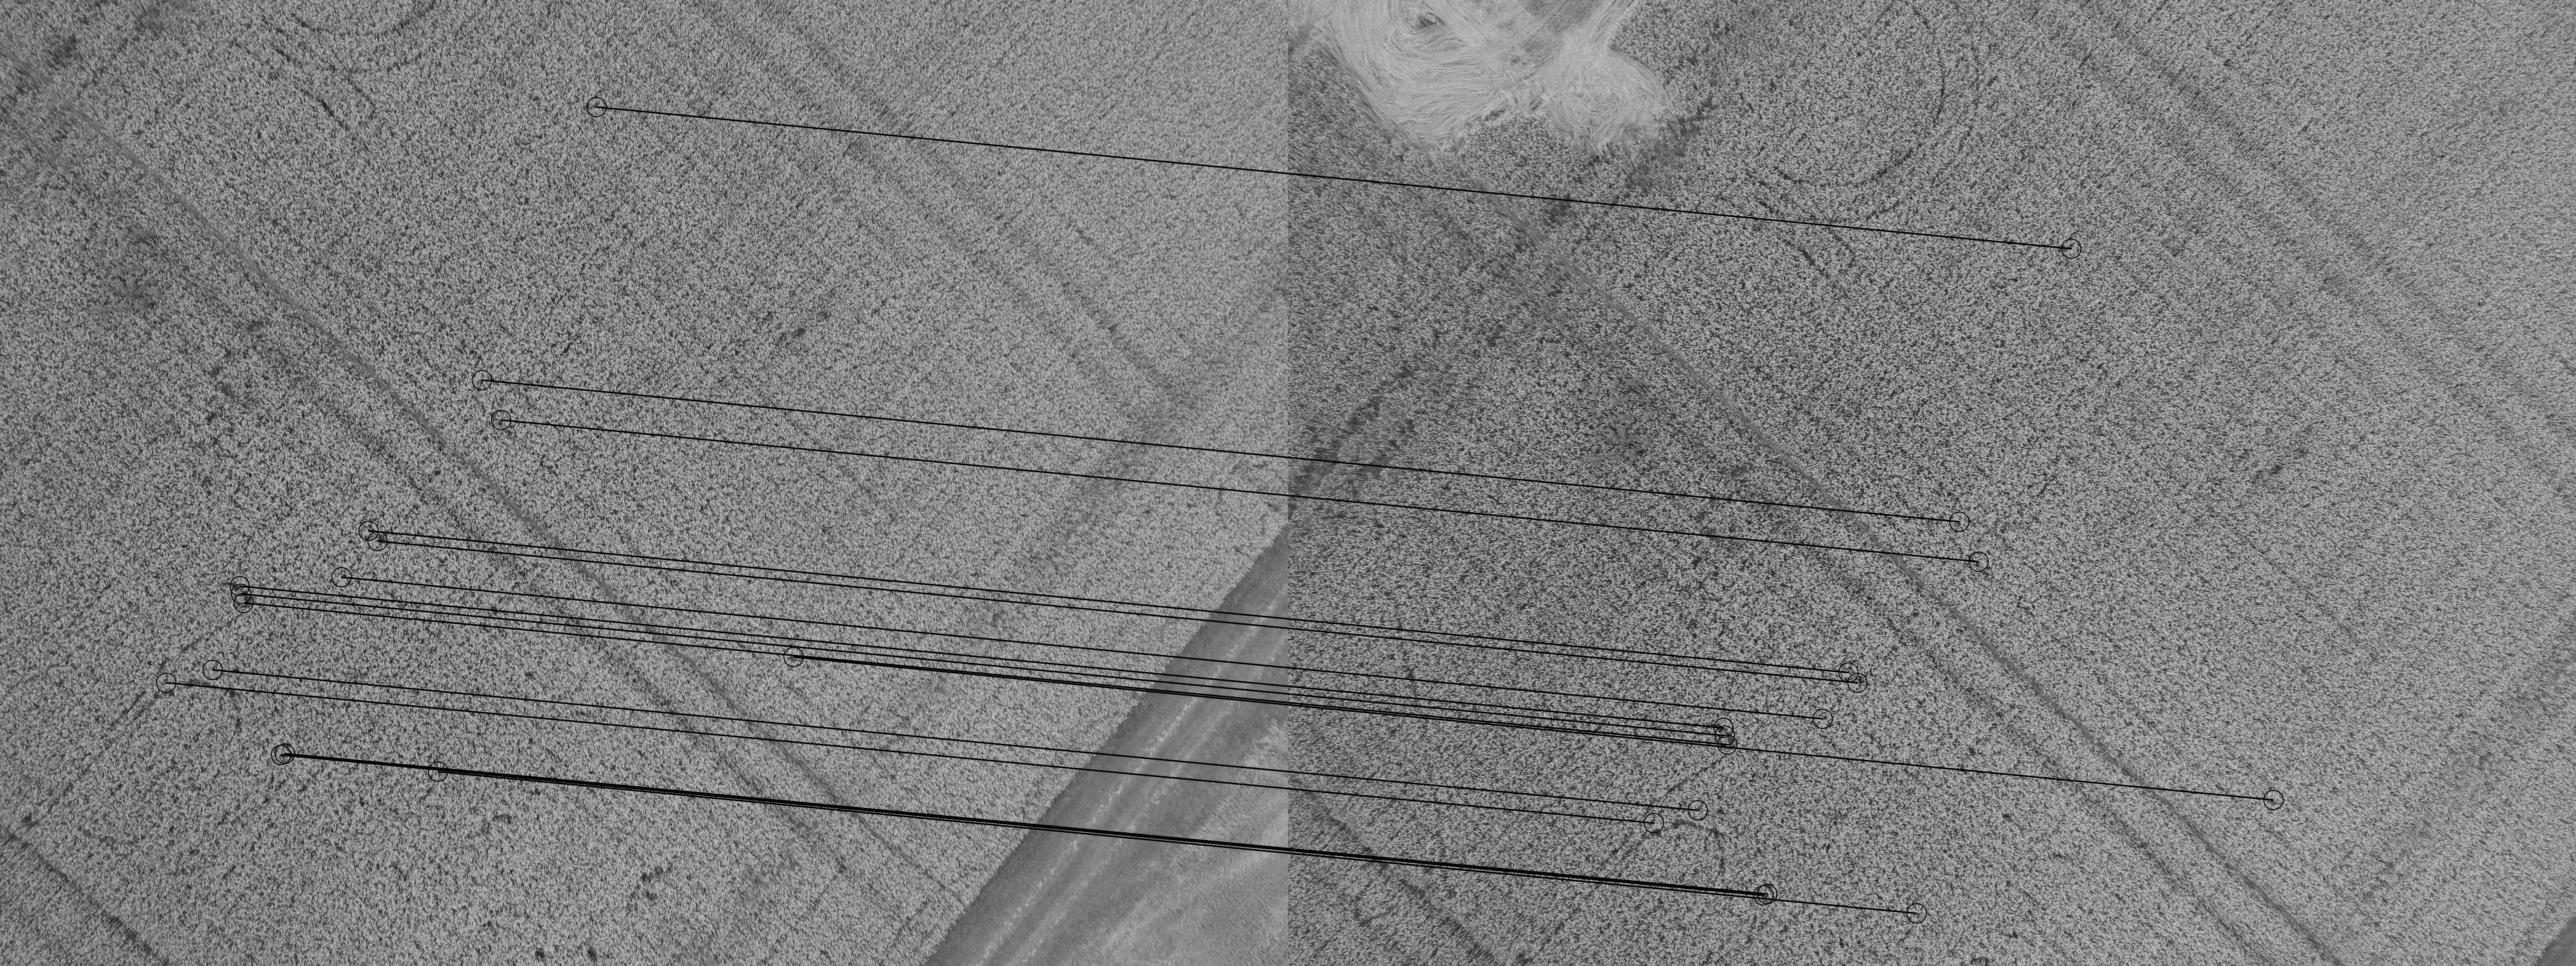
\includegraphics[width=1.11\textwidth]{fig/10best-HarrisSift-octave1.jpg}
    \vspace{-0.5em}   
    \begin{center}
    \caption{\textcolor{gray}{\footnotesize \textit{
    Tre lyse blobs på en mørk baggrund illustreret i 2 dimensioner \cite{blob}}}}
    \label{fig:lindblob}
     \end{center}
  \end{figure}
       \vspace{-2.7em}
\noindent





\section{SIFT}
\begin{figure}[H]
    \centering
    \begin{center}    
    \begin{tabular}{ | l | l | l | l | l | l | l |}
    \hline
    Filename 1 & Filename 1 & |$\bold{A}$| & |$\bold{A'}$| & $mean(A,A')$ & $Match(\bold{A}, \bold{A}')$ & $Rm$ \\ \hline
IMG\_9370.jpg &	IMG\_9371.jpg &	10914 &	13590 &	12252.0 &	237 &	0.0193\\ \hline
IMG\_9371.jpg &	IMG\_9372.jpg &	13590 &	14457 &	14023.5 &	351 &	0.0250\\ \hline
IMG\_9372.jpg &	IMG\_9373.jpg &	14457 &	10146 &	12301.5 &	152 &	0.0123\\ \hline
IMG\_9373.jpg &	IMG\_9374.jpg &	10146 &	9625 &	9885.5 &	100 &	0.0101\\ \hline
IMG\_9374.jpg &	IMG\_9375.jpg &	9625 &	10288 &	9956.5 &	184 &	0.0184\\ \hline
IMG\_9375.jpg &	IMG\_9376.jpg &	10288 &	11735 &	11011.5 &	266 &	0.0241\\ \hline
IMG\_9376.jpg &	IMG\_9377.jpg &	11735 &	10455 &	11095.0 &	345 &	0.0310\\ \hline
IMG\_9377.jpg &	IMG\_9378.jpg &	10455 &	9026 &	9740.5 &	271 &	0.0278\\ \hline
IMG\_9378.jpg &	IMG\_9379.jpg &	9026 &	9095 &	9060.5 &	567 &	0.0625\\ \hline
IMG\_9379.jpg &	IMG\_9380.jpg &	9095 &	7545 &	8320.0 &	509 &	0.0611\\ \hline
    \end{tabular}       
    \caption{\textcolor{gray}{\footnotesize \textit{Fire forskellige oktaver, og filterstørrelse, for et andenafledt filter}}}
    \label{tab:SURFOCTAVE2}
     \end{center}
     \vspace{-2.5em}
\end{figure} \noindent
Middelværdi af repeatability mesaure = 0.0292

\begin{figure}[H]
    \centering
    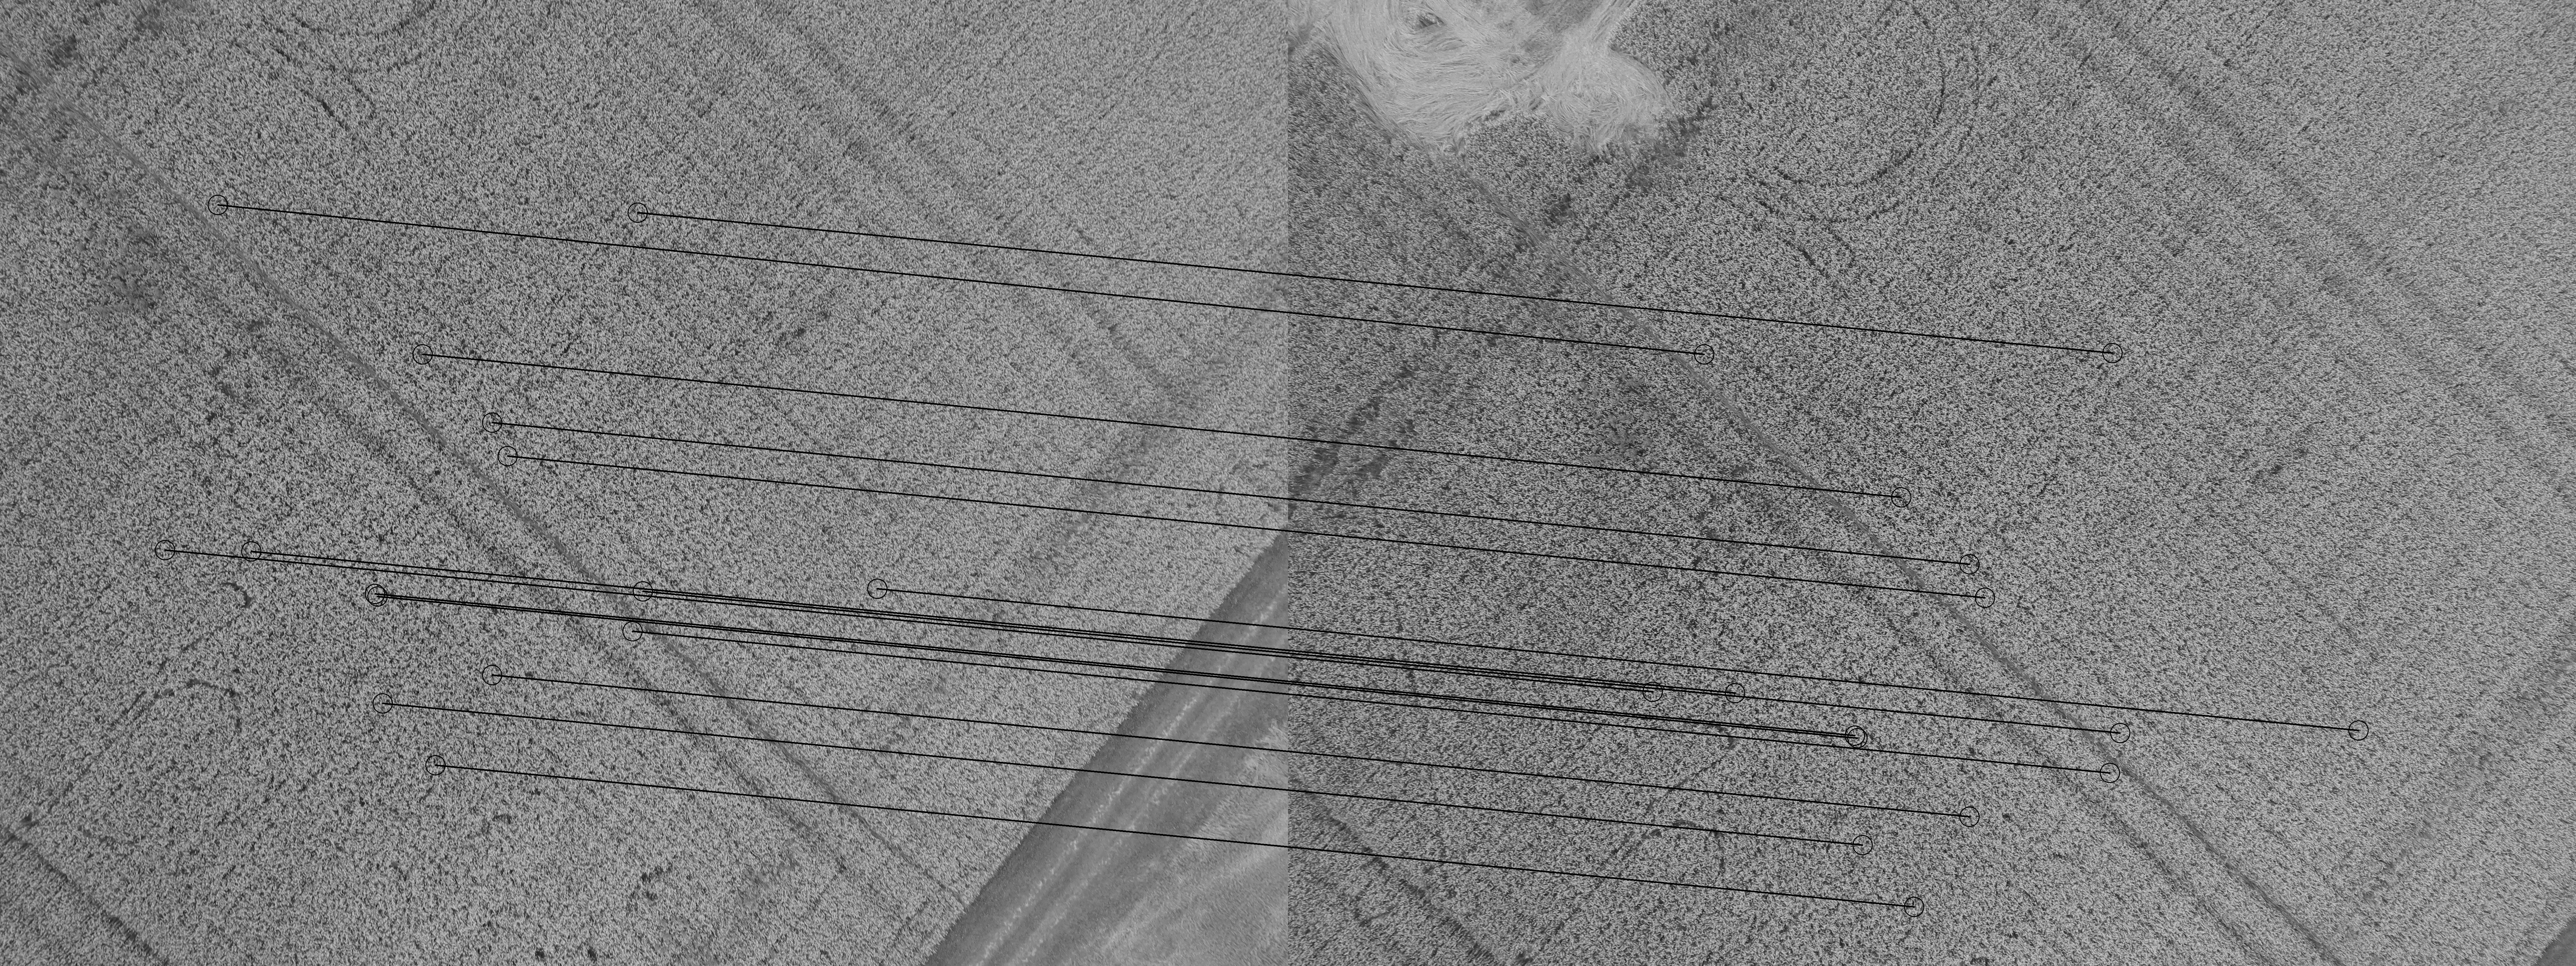
\includegraphics[width=1.11\textwidth]{fig/10best-SIFT-octave2.jpg}
    \vspace{-0.5em}   
    \begin{center}
    \caption{\textcolor{gray}{\footnotesize \textit{
    Tre lyse blobs på en mørk baggrund illustreret i 2 dimensioner \cite{blob}}}}
    \label{fig:lindblob}
     \end{center}
  \end{figure}
       \vspace{-2.7em}
\noindent





\section{SURF}
\begin{figure}[H]
    \centering
    \begin{center}    
    \begin{tabular}{ | l | l | l | l | l | l | l |}
    \hline
    Filename 1 & Filename 1 & |$\bold{A}$| & |$\bold{A'}$| & $mean(A,A')$ & $Match(\bold{A}, \bold{A}')$ & $Rm$ \\ \hline
IMG\_9370.jpg &	IMG\_9371.jpg &	12529 &	12882 &	12705.5 &	3249 &	0.2557\\ \hline
IMG\_9371.jpg &	IMG\_9372.jpg &	12882 &	14700 &	13791.0 &	3422 &	0.2481\\ \hline
IMG\_9372.jpg &	IMG\_9373.jpg &	14700 &	14636 &	14668.0 &	557 &	0.0379\\ \hline
IMG\_9373.jpg &	IMG\_9374.jpg &	14636 &	14352 &	14494.0 &	622 &	0.0429\\ \hline
IMG\_9374.jpg &	IMG\_9375.jpg &	14352 &	13902 &	14127.0 &	566 &	0.0400\\ \hline
IMG\_9375.jpg &	IMG\_9376.jpg &	13902 &	12200 &	13051.0 &	2575 &	0.1973\\ \hline
IMG\_9376.jpg &	IMG\_9377.jpg &	12200 &	11614 &	11907.0 &	2800 &	0.2351\\ \hline
IMG\_9377.jpg &	IMG\_9378.jpg &	11614 &	10028 &	10821.0 &	1005 &	0.0928\\ \hline
IMG\_9378.jpg &	IMG\_9379.jpg &	10028 &	10600 &	10314.0 &	1911 &	0.1852\\ \hline
IMG\_9379.jpg &	IMG\_9380.jpg &	10600 &	9955 &	10277.5 &	1761 &	0.1713\\ \hline
    \end{tabular}       
    \caption{\textcolor{gray}{\footnotesize \textit{Fire forskellige oktaver, og filterstørrelse, for et andenafledt filter}}}
    \label{tab:SIFTOCTAVE3}
     \end{center}
     \vspace{-2.5em}
\end{figure} \noindent
Middelværdi af repeatability mesaure = 0.2342


\begin{figure}[H]
    \centering
    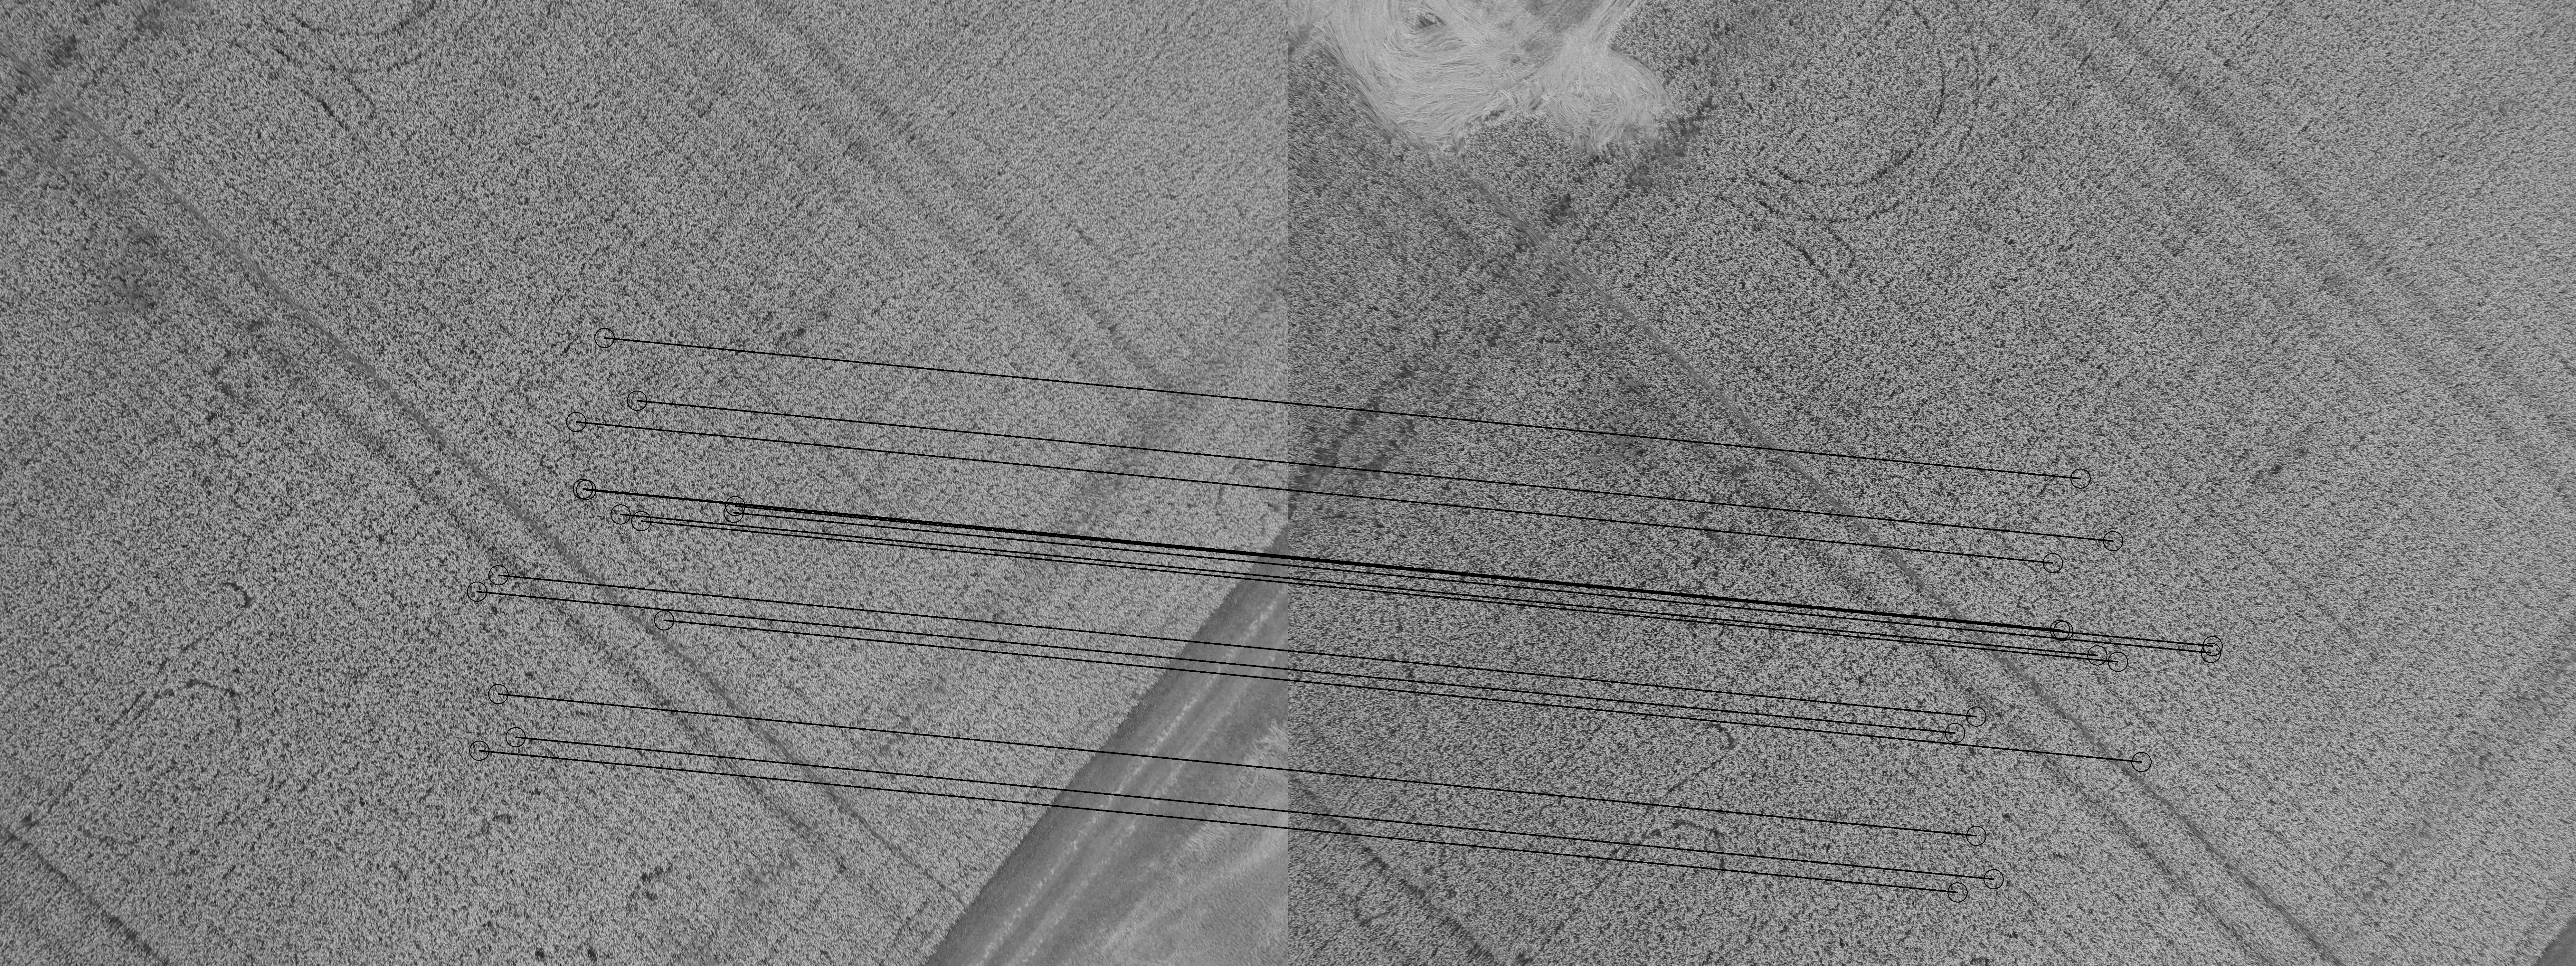
\includegraphics[width=1.11\textwidth]{fig/10best-SURF-octave3.jpg}
    \vspace{-0.5em}   
    \begin{center}
    \caption{\textcolor{gray}{\footnotesize \textit{
    Tre lyse blobs på en mørk baggrund illustreret i 2 dimensioner \cite{blob}}}}
    \label{fig:lindblob}
     \end{center}
  \end{figure}
       \vspace{-2.7em}
\noindent



\section{Diskussion}
